\documentclass{resonance}
\usepackage{textgreek}
\usepackage{lipsum}
\usepackage{newpxtext,newpxmath}
\usepackage{algorithm2e}
\NoCaptionOfAlgo
\usepackage{tcolorbox}
\usepackage{mathrsfs}
\usepackage{bm, amsbsy}
\usepackage{xcolor}
\usepackage[hidelinks=true]{hyperref}

\definecolor{greenish}{RGB}{141,198,63}
\definecolor{reddish}{RGB}{239,65,54}
\definecolor{blueish}{RGB}{0, 153, 221}
\definecolor{alg1}{RGB}{122,89,239}
\definecolor{alg2}{RGB}{9, 166, 75}
\definecolor{alg3}{RGB}{124,198,137}

\hypersetup{
colorlinks   = true, %Colours links instead of ugly boxes
urlcolor     = blueish, %Colour for external hyperlinks
linkcolor    = reddish, %Colour of internal links
citecolor   = greenish %Colour of citations
}

\def\e{\text{e}}
\def\eb{\mathbf{e}}
\def\grad{\nabla}
\def\at{\hat{a}}
\def\Ai{\mathcal{A}}
\def\J{\mathcal{J}}
\def\R{\mathbb{R}}
\def\d{\text{d}}
\def\E{\mathbb{E}}
\def\x{\bm{\theta}}
\def\th{\bm{\theta}}
\def\thh{\bm{\hat{\theta}}}
\def\y{\bm{y}}
\def\yh{\bm{\hat{y}}}
\def\n{\bm{n}}
\def\z{\mathbf{z}}
\def\f{\bm{f}}
\def\w{\mathbf{w}}
\def\q{\mathbf{q}}
\def\r{\mathbf{r}}
\def\m{\bm{m}}
\def\p{\bm{\beta}}
\def\K{\bm{\kappa}}
\def\T{\mathsf{T}}
\def\S{\bm{\sigma}}
\def\H{\bm{\alpha}}
\def\J{\mathcal{J}}
\def\I{\mathbb{I}}
\def\A{\mathcal{A}}
\def\B{\mathcal{B}}
\def\O{\mathcal{O}}
\def\E{\mathbb{E}}
\def\eps{\bm{\epsilon}}
\def\PhiB{\boldsymbol{\Phi}}
\def\GammaB{\boldsymbol{\Gamma}}
\def\LambdaB{\boldsymbol{\Lambda}}
\def\xh{\hat{\bm{x}}}



\def\tcb@proc@counter@auto#1{%
  \newcounter{tcb@cnt@#1}%
  \csxdef{tcb@cnt@#1}{tcb@cnt@#1}%
  \tcb@proc@counter@autoanduse{#1}%
  \ifcsname resetcounteronoverlays\endcsname%<-added
  \resetcounteronoverlays{tcb@cnt@#1}%<-added
  \fi%<-added
}
\makeatother

\newtcolorbox[auto counter]{egsBox}[2][]{%
colback=alg2!10,colframe=alg2!70,center, fonttitle=\bfseries, title=Example~\thetcbcounter: #2,#1}

\newtcolorbox[auto counter]{algBox}[2][]{%
colframe=alg1!70,colback=alg1!10,center, fonttitle=\bfseries, title=Algorithm~\thetcbcounter: #2,#1}

\begin{document}
\title{Part 1: Revisiting linear filtering, the Bayesian paradigm \& optimal state estimation}
\secondTitle{From least-squares to Kalman filter}
\author{S Ganga Prasath, Vishaal Krishnan}

\maketitle

\authorIntro{\includegraphics[width=2cm]{./figs/sgp.jpg}\\
S Ganga Prasath is currently a visiting faculty in the Department of Applied Mechanics, Indian Institute of Technology Madras, Chennai. His research interest lies at the intersection of robotics and behavior.\\[10pt]
\includegraphics[width=2cm]{./figs/vishaal.jpg}\\
Vishaal krishnan is a post-doctoral researcher in the School of Engineering and Applied Sciences, Harvard University, Cambridge. His research interests are in control theory, cognition and navigation.}

%%abstract
\begin{abstract}
In this two part series, we discuss the theoretical underpinnings of two important control-theoretic formalisms: $(i)$ optimal state-estimation; $(ii)$ optimal control, with a tutorial approach. The Kalman filter is a classical technique for optimal state-estimation for linear systems, the purpose of which is to make the best possible quantitative estimates of the underlying system state from fluctuating measurements given the knowledge of the system's behavior as well as the measurement process. Its manifold applications, ranging from molecular imaging to aerospace engineering, has given it landmark status within control theory, while its foundations are rooted in the least-squares method accessible at the undergraduate level. Given its enormous utility, it is surprising to note that these ideas have not percolated into several other fields. In this article, we walk the reader through the calculation of the filtering technique, borrowed from well-known texts in the control theory literature.
\end{abstract}


\section{Introduction}
Linear dynamical systems with constant coefficients capture numerous physical phenomena and are the simplest form of differential equations that often reside in the pages of undergraduate textbooks. The solution to these dynamical systems have either growing, decaying, oscillating, saturating\keywords{least-squares method, Kalman filter, state-estimation problem etc.} or stationary behavior depending on the constants in the system and the initial conditions pertaining to their dynamics. Even in these simple systems, experimentally making quantitative estimates of the constants involved in the dynamics can be daunting. This is a common problem in engineering and is given the name, as one would expect, the \textit{state-estimation} problem. The primary motivation behind this problem is to make the best possible estimate of a state-vector that captures the dynamics (or the constants) of the system. A more challenging task is to make these estimates in a fluctuating environment that adds to the uncertainty in the measurements. One of the landmark results in control theory, the field that studies such problems, is the exact solution of the best/optimal estimate (which will define soon) of the state-vector and is given by the name \textit{Kalman filter} (denoted as KF from now on)~\cite{kalman1960new}.

In this pedagogical tutorial, we will look at the derivation of the Kalman filter for discrete linear dynamical system whose basic idea comes from the illustrious least-squares estimation problem. Following this, we briefly discuss the formal solution to the estimation problem for linear continuous dynamical systems i.e. the Kalman-Bucy filter~\cite{kalman1961new} and highlight how the Kalman filter fits naturally in the Bayesian paradigm. We show examples throughout the article to make the approach and the notation transparent, building up to the ultimate problem of estimation of the position of a brownian particle in a harmonic trap. There is a supplementary \href{https://github.com/sgangaprasath/KFTutorial/blob/main/KFTutorial.ipynb}{\texttt{python}}-code that goes with this tutorial with the numerical implementation of these algorithms. We leave the reader with a partial list of applications stampeded by Kalman/-Bucy filters and some of the open questions related to Kalman filter. The details of the calculation, the format of presentation and examples are heavily borrowed from well known texts~\cite{stengel1994optimal, sorenson1970least, maybeck1982stochastic}.

\begin{figure}
    \centering
    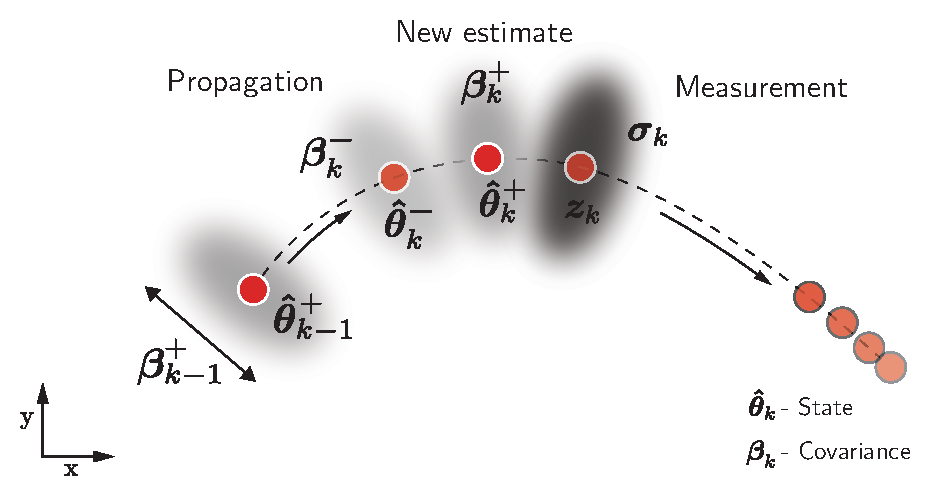
\includegraphics[width=0.9\textwidth]{./figs/KFSchematic.pdf}
    \caption{Schematic showing the 3 steps involved in Kalman filtering for the case of a simple projectile motion where the state is the position \& velocity of the ball (whose estimates are denoted by the vector $\thh_k$ and the covariance by $\p_k$). The 3 steps being: $(i)$ estimate propagation, $\thh_k^{-}, \p_k^{-1}$; $(ii)$ measurement, $\z_k$ (with its covariance $\S_j$), $(iii)$ state-estimate and covariance estimate update $\thh_k^{+}, \p_k^{+}$.}
    \label{fig:KFschm}
\end{figure}

\section{Stochastic linear dynamical systems}\label{sec:sde}
Before we look at the steps leading to the derivation of the Kalman filter, we take a quick tour of stochastic differential equations (SDEs) and their properties that will be relevant to our derivation. Stochastic dynamical systems are different from simple dynamical systems in that the dynamical variable is subjected to a source of noise (which have often singular, non-differentiable properties). The solution to these equations can be thought of as a continuous random variable capturing a process i.e. \textit{stochastic process}~\cite{balakrishnan2008elements}. Consider a stochastic dynamical system in $\x(t) \in \R^d$ with white noise $\w(t) \in \R^d$ given by
\begin{align}
\d \x(t) =& \ \f(t) \x(t) \ \d t + \d \w(t), \label{eq:sdeEq} \\
\E [\w(t)] =& \ 0, \\
\E [\w(t) \w^\T(\tau)] =& \ \q(t) \delta (t-\tau).
\end{align}

Here $\f(t)$ is a known function of time, $\w(t)$ is the zero-mean Gaussian random variable and $\q(t)$ is its correlation (see Egs.~\ref{egs:sde} for details). The evolution of the mean of the state vector $\x(t)$, defined by $\E[\x] = \m(t) $, can be written as $ \dot{\m}(t) = \f(t) \m(t)$, and the variance $\E[(\x - \m)(\x - \m)^\T] = \p(t)$ can be written as $\dot{\p}(t) = \f(t) \p(t) + \p(t) \f^\T(t) + \q(t)$. Here $\E[\bullet]$ denotes an ensemble average where several realizations of the same stochastic differential equation in Eq.~\ref{eq:sdeEq} are used to obtain an average of the quantity in brackets. In 1-dimension when $\f(t)$ is a constant, $f(t) = -\gamma$, such that $\gamma > 0$, the solution $\th(t)$ is called an Ornstein-Uhlenbeck process and when $\f(t) = 0$, the solution is that of brownian motion. In Egs.~\ref{egs:sde} we look at the evolution of a simple SDE whose evolution can calculated analytically and provide a  a numerical implementation in the \href{https://github.com/sgangaprasath/KFTutorial/blob/main/KFTutorial.ipynb}{\texttt{python}}-code.

\begin{figure}
    \centering
    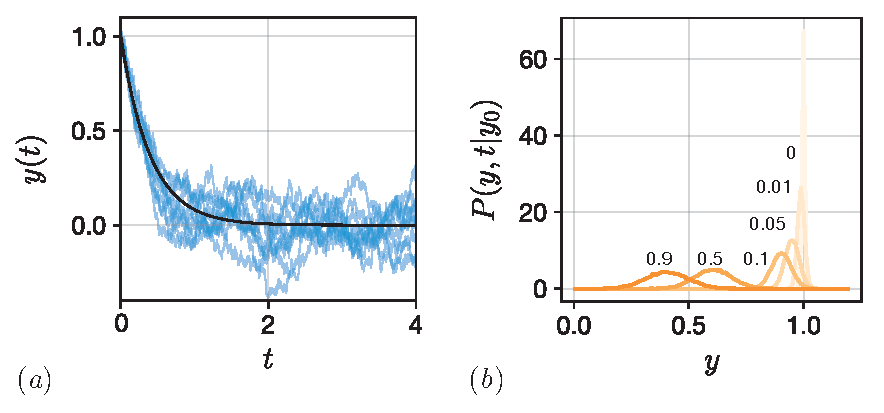
\includegraphics[width=\textwidth]{./figs/sde.pdf}
    \caption{$(a)$ Time evolution of $y(t)$ (in green) for different trial when $y_0=1$, $a=-1$ and $D=10^{-2}$ in Egs.~\ref{egs:sde}. The solid line shows the mean $m(t)$ which is simply $m(t) = m_0 \exp(at)$. $(b)$ Temporal evolution of the probability density function $P(y,t)$ shown at different time instants (indicated above the curve), computed from several runs of the same SDE starting at $y_0=1.0$. Refer to the \href{https://github.com/sgangaprasath/KFTutorial/blob/main/KFTutorial.ipynb}{\texttt{python}}-notebook for further details.}
    \label{fig:sdeFig}
\end{figure}

When we move from continuous dynamical system to discrete system, the discrete version of the average equations can also be derived given the underlying evolution of $\x_k$ (where $k$ denotes the $k$-th step). A discrete linear dynamical system in $\x_k$ can be written as
\begin{align}
\x_k =& \ \PhiB_{k-1} \x_{k-1} + \LambdaB_{k-1} \w_{k-1}.
\end{align}

Here $\PhiB_k$ is the propagator that evolves $\x_{k-1}$ to $\x_k$ and $\LambdaB_{k}$ is the amplitude of noise. The white noise has the property $\E[\w_k] = 0, \E[\w_k \w_l^\T] = \q_k \delta_{k,l}$ where $\delta_{k,l}$ is the Kronecker delta function. With this the evolution of the mean then becomes $\E[\x_k] = \m_k = \PhiB_{k-1} \m_{k-1}$ and the variance can be written after little algebra as $\p_k = \PhiB_{k-1} \p_{k-1} \PhiB_{k-1}^\T + \LambdaB_{k-1}\q_{k-1}\LambdaB^\T_{k-1}$ where $\p_k = \E[(\x_k-\m_k)(\x_k-\m_k)^\T]$ is the covariance matrix. We see that provided the initial probability distribution of the state vector i.e. $\thh_0$ (or its mean $\m_0$ and variance $\p_0$), the evolution of $\thh_k$ can be computed provided $\PhiB_k,  \LambdaB_k$ are given for $k=1 \dots n$.

\begin{egsBox}[label={egs:sde}]{Evolution of a simple 1D SDE}
\footnotesize
Consider a simple dynamical system $\dot{y}(t) = a y(t) + b$ with $a, b \in \R$ being constants. This has a solution of the form $y(t) = [-b + (a y_o + b) \e^{a t}]/a$ where the initial condition is $y(0) = y_o$. We see that there are 3 parameters in the system i.e. $a, b$ and $y_o$ that determine the dynamics. When this dynamics is superposed with stochastic noise, the evolution can be written as a SDE of the form $\d y(t) = a y(t) \ \d t + \d w(t)$ where $w(t)$ is white noise. The white noise is a random sequence is characterized by $\E [w(t)] = 0$ and the correlation is given by $\E[w(t)w(\tau)] = q \delta(t-\tau)$. The magnitude of the correlation is often set to $q=2D$ where $D$ is the diffusion coefficient.

We know from sec.~\ref{sec:sde} that the mean evolves as $\dot{m}(t) = a m(t)$ which has solution $m(t) = m_0 \exp{a t}$ and covariance evolves as $\dot{\beta}(t) = 2 a \beta(t) + 2D$ whose solution is $\beta(t) = -D/a( 1 - \exp{(2at)} )$. However, the SDE (called the Langevin equation, capturing the Ornstein-Uhlenbeck process) has a formal solution $y(t) = y_0 \exp{a t} + \int_0^t \exp{a(t-s)}\ \d w(s) $ and is valid for $a < 0$. Moreover, we can write the evolution of the $P(y,t|y_0)$ which is the probability of finding $y$ at time $t$ starting at $y_0$ (which is the corresponding Fokker-Plack equation whose details we don't go over here, refer~\cite{chandrasekhar1943stochastic, balakrishnan2008elements}) as
\begin{align*}
    P(y,t|y_0) = \frac{1}{\sqrt{2 \pi D (\e^{2 a t} - 1)/a}} \exp \bigg[- \frac{(y-y_0\e^{at})^2}{2D(\e^{2 a t} - 1)/a} \bigg].
\end{align*}
In Fig.~\ref{fig:sdeFig}$(a)$ we show the dynamics of $y(t)$ obtained by numerically simulating the Langevin equation and in Fig.~\ref{fig:sdeFig}$(b)$ the probability density function $P(y,t|y_0)$ computed by simulating several trials. The \href{https://github.com/sgangaprasath/KFTutorial/blob/main/KFTutorial.ipynb}{\texttt{python}}-notebook has further details of the implementation.
\end{egsBox}

\section{Least-squares estimation} \label{sec:lse}
We start with the derivation of the least-squares estimator (shortened as LSE hereafter) using which we can fit a model to data by minimizing the error between the model and the data. Least-squares fit/estimator has a long history and dates back to the days of the then young Karl Friedrich Gauss in 1795.  Gauss used the least-squares estimator that he had developed to calculate the parameters necessary to describe the motion of the comet Ceres from astronomical measurements. Using this he managed to predict the time when the comet would reappear from behind the sun’s glare and win the competition set by the Italian astronomer Giuseppe Piazzi. Gauss being the inventor of the least-squares method, however, was not apparent during his days and it involves a fascinating anecdote between him and Legendre.\leftHighlight{Least-squares estimation dates back to the days of Gauss in 1795. He used it to win the competition set by the Italian astronomer Giuseppe Piazzi by predicting the time when a comet would reappear from behind the sun’s glare.} We direct the interested readers to~\cite{sorenson1970least} for a detailed summary. A least-squares estimator provides the best possible fit to the data assuming that we are aware of the model that generated the data. In the example of Gauss, he already had the model of the comet's motion from initial measurements of its trajectory. The notion of best possible fit implies that the error between the data generated by the model and that of the measured data is minimized. In general, we know that models of physical systems involve physical parameters and that the primary motivation behind this estimation process is to come up with values or estimates of these parameters. To keep this simple, we look at an example where the model is a linear function of the parameters. In general when the model is a non-linear function of the parameters, more complex properties of the fit arise (see~\cite{transtrum2015perspective} for further details) and details of such fits are well outside the domain of interest of this tutorial.

In order to state things more concretely in mathematical form, let us consider a dynamical 1-dimensional trajectory of a particle $y(t; \th) \in \R$ which is a function of time $t$ and set of parameters $\theta_i \in \R$ where $i = 1\dots k$, denoted using vector $\th \in \R^k$ that are the physical constants and/or the initial conditions (depending on the details of the system we are interested). As the trajectory is a linear function of the parameters, we can write $y(t) = \f(t)^\T \th$ where $\f(t)$ is often called the feature vector or template vector containing the functional form of basis functions/model to which we would like to fit the data. We make discrete measurements of the particle trajectory at time instants $t_i$ where $i = 1\dots n$ to obtain a vector $\m \in \R^n$.

\begin{egsBox}[label=egs:lse]{Least square estimation of constants for a one-dimensional trajectory}
\footnotesize
Consider a time-varying trajectory of a particle in 1D given by $y(t) = a t + b t^{3/2} + c t^2 + d t^4$. From this we can write $\f(t) = [ t\ t^{3/2}\ t^2\ t^4]$ and the state $\th = [ a, b, c, d]$. From this we can immediately compute the $\H = \f(t_i)$ matrix of dimensions $n \times 4$ after $n$-measurements at $t = \Delta t [ 1, 2, \dots, n]$. We can compute the measurement $\m \in \R^{n \times 1}$ from data collected at discrete time-instants $t_j$ if we know the distribution of the noise that corrupted the data.

Assuming that $\n \sim \mathcal{N}(0,1)$ where $\mathcal{N}(\mu, \sigma)$ is the normal distribution with mean $\mu$ and standard deviation $\sigma$, we now have the model matrix $\alpha$ and the measurement $\m$ which is all we require to compute the estimation of $\th$ given by $\thh = (\H^\T \H)^{-1} \H^\T \m$. We show in Fig.~\ref{fig:lseFig}$(a)$ the comparison between the measurements and the solution trajectory obtained by using the estimated constants from least squares method. In Fig.~\ref{fig:lseFig}$(b)$ we show that the error in computed constants (defined by $||\th-\thh||$) goes to zero with increase in number of measurements $n$. The reader is strongly encouraged to look at the \href{https://github.com/sgangaprasath/KFTutorial/blob/main/KFTutorial.ipynb}{\texttt{python}}-code that goes with the article for details.
\end{egsBox}

The first assumption we make about the measurement process is that the measurement is a linear function of the state and is corrupted by a noise $\n$ (due to environmental fluctuations or sensor noise): $\m = \H \th + \n$ where $\H = \f(t_i) \in \R^{n \times k}$. Just to be clear, we now have access to $\H$ (because we know the functional form of the model $\f(t)$) and $\m$ (which is the actual measurement) but not $\th$. Our aim is to make the best estimate of $\th$ which we denote by $\thh$ given $\H, \m$. 

\subsubsection*{Residual error minimization}
Although our motivation is to minimize the error $||\th - \thh||$, we do not have access to $\th$. So our best estimate has to be based on $\m$ and $\yh$ where $\yh = \H \thh$. We can define the error $\eps = (\m - \yh)$ (also called the \textit{measurement residual}) and from this the quadratic cost function is given by
\begin{align*}
\J(\thh) =& \ \frac{1}{2}\eps^\T \eps = \frac{1}{2} (\m - \yh)^\T (\m - \yh) \\
=& \ \frac{1}{2}  (\m^\T \m - \m^\T\H\thh - \thh^\T \H^\T \m + \thh^\T \H^\T \H \thh),
\end{align*}
which can be minimized by setting
\begin{align*}
\frac{\delta \J(\thh)}{\delta \thh} =& \ (\H^\T\H \thh - \H^\T \m)^\T = 0.
\end{align*}
\leftHighlight{Minimizing the measurement error, the solution to the least square estimation problem to compute $\th$ is $\thh =  (\H^\T \S^{-1} \H)^{-1} \H^\T \S^{-1} \m$ where $\H$ is the model, $\S$ is a weight matrix (often the covariance of the error).} We see that the best estimate of $\th$ is $\thh = (\H^\T \H)^{-1} \H^\T \m$. We can easily show that $\delta^2 \J(\thh)/\delta \thh^2 = \H^\T \H$ which is positive definite providing the sufficiency condition that the solution obtained is a minimum. When you know more about the noise in the measurement process, one can also obtain an appropriately weighted estimate $\thh$ with a weight matrix $\S$ to get $\thh =  (\H^\T \S^{-1} \H)^{-1} \H^\T \S^{-1} \m$ where $\S$ is the co-variance of the noise. In Egs.~\ref{egs:lse} we look at an example problem where we deploy the fit derived here and  Fig.~\ref{fig:lseFig} shows a sample fit.

\subsubsection*{Direct least-squares}
If in addition to the description of the measurement process $\m = \H \th + \n$, when we have prior knowledge of the covariance of the parameters $\th$, we can seek to directly minimize the squared error $\left\| \hat{\th} - \th \right\|^2$ of the estimate $\hat{\th}$ on an average.
Just as in the case of (measurement) residual error minimization,
we seek an estimate $\hat{\th}$ that is a linear function of 
the measurement $\m$, i.e., $\hat{\th} = \K \m$ (where $\K \in \R^{k \times n}$ is called the \textit{gain} and will play an important role later) by solving the following minimization problem
\begin{align*}
    \min_{\K} \mathbb{E} \left[ \left\| \hat{\th} - \th \right\|^2 \right].
\end{align*}
Here $\E[\bullet]$ denotes average over several trials of measurement of the same particle dynamics, just as described in sec.~\ref{sec:sde} Substituting the model $\hat{\th} = \K \m$ above, we obtain
\begin{align*}
    \min_{\K} \mathbb{E} \left[ \left\| \hat{\th} - \th \right\|^2 \right] &= \min_{\K} \mathbb{E} \left[ \left\|  \K \m - \th \right\|^2 \right] = \min_{\K} \mathbb{E} \left[ \left\|  \K (\H \th + \n) - \th \right\|^2 \right].
\end{align*}
Expanding the above equation, we get
\begin{align*}
    \min_{\K}  \mathbb{E} \left[ \th^\top ( \K \H - \I )^\top ( \K \H - \I ) \th + 2 \th^\top ( \K \H - \I )^\top \K \n 
    + \n^\top \K^\top \K \n \right].
\end{align*}
Note that the individual terms in the cost above are 
scalar inner products which can be rewritten as the
trace of the corresponding outer products as follows
\begin{align*}
    \min_{\K}  \mathbb{E} \bigg[ \ \mathrm{Tr} \{ ( \K \H - \I ) \th \th^\top ( \K \H - \I )^\top  + 2 \K \n \th^\top ( \K \H - \I )^\top  + \K \n \n^\top \K^\top  \} \bigg].
\end{align*}
\leftHighlight{Minimizing the mean-squared error on the parameter estimate, the solution to the direct least-squares estimation problem to compute $\th$ is $\thh = \p \H^\top \left( \H \p \H^\top + \S \right)^{-1} \m$ where $\H$ is the model, $\p$ is the covariance of the true parameter $\th$ and $\S$ is the covariance of the noise.}From the commutativity of the expectation and trace operations
and the fact that $\th$ and $\n$ are independent
random variables, the above reduces to
\begin{align*}
    &\min_{\K} \mathrm{Tr} \left\lbrace ( \K \H - \I ) \mathbb{E} \left[  \th \th^\top \right] ( \K \H - \I )^\top  + \K \mathbb{E} \left[ \n \n^\top \right] \K^\top  \right \rbrace \\
    &= \mathbb{E} [  \th \th^\top ] + \min_{\K} \mathrm{Tr} \lbrace \K ( \H  \mathbb{E} [  \th \th^\top ]  \H^\top \\
    &\  + \mathbb{E} [ \n \n^\top ] ) \K^\top  - 2 \K \H \mathbb{E} [  \th \th^\top ] \rbrace.
\end{align*}

Taking the covariances of $\th$ and $\n$ to be $\p = \E[\th \th^\T] \in \R^{k\times k}$
and $\S=\E[\n\n^\T] \in \R^{n\times n}$ respectively, and setting the first variation with
respect to $\K$ of the cost above to zero,
we get the optimal $\K$ (denoted by $\K^*$) as
\begin{align*}
    \K^* = \p \H^\top \left( \H \p \H^\top + \S \right)^{-1},
\end{align*}
and the optimal estimate then becomes
\begin{align*}
    \hat{\th} =  \p \H^\top \left( \H \p \H^\top + \S \right)^{-1} \m.
\end{align*}

\begin{figure}
    \centering
    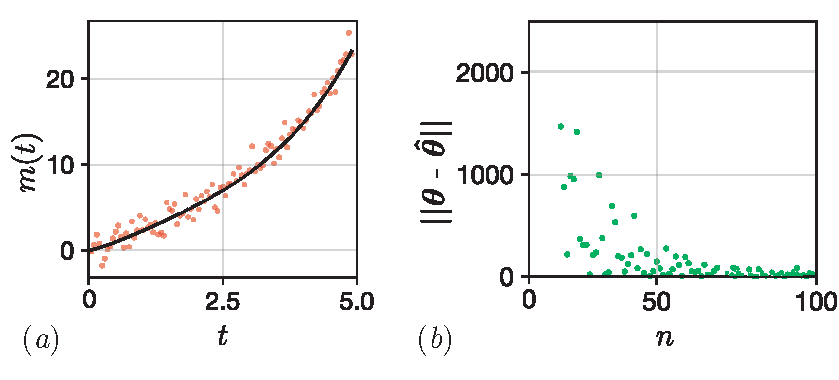
\includegraphics[width=\textwidth]{./figs/lse.pdf}
    \caption{$(a)$ Comparison between measurements $\m(t_i)$ and the trajectory $\yh(t)$ (solid black line) obtained by least square estimation. $(b)$ $L_2$-norm of error in computed constants defined as $||\th - \thh ||$ as a function of the number of measurements $n$.}
    \label{fig:lseFig}
\end{figure}

\subsubsection*{Recursive least-square estimator}
The next step towards the derivation of the Kalman filter is to make estimate of the state $\thh$ as and when the data is collected instead of assuming that the measurement is a fixed vector. The estimator we derive in this subsection is called the \textit{recursive least-square estimator} (shortened as RLSE). Let us consider the situation when we have collected $n_1$ measurements of the same dynamical process as earlier, given by $\m_1 \in \R^{n_1}$ and make an estimate $\thh_1$. We know from our current algorithm that, this is given by $\thh_1 =  (\H_1^\T \S_1^{-1} \H_1)^{-1} \H_1^\T \S^{-1} \m_1$ where $\H_1 = \f(t_i) \ \forall \ t_i, i = 1 \dots n_1 \in \R^{n_1 \times k}$. We would like to update $\thh_1 \in \R^{k}$ when more measurements are made. Now new measurements $\m_2 \in \R^{n_2}$ are made such that $\H_2 =  \f(t_i) \ \forall \ t_i, i = n_1+1 \dots n_1+n_2 \in \R^{(n_1+n_2) \times k}$. With this new measurement, the new estimate that minimizes over entire error using both $\m_1, \m_2$ is given by $\thh_2$. Assuming that we know the measurement error covariance for both the steps, $\S_j=\E[\n_j\n_j^\T]$, we can write the total error as
\begin{align}
\J(\m_1, \m_2) =& \ [ (\m_1-\H_1 \thh_2)^\T \ (\m_2-\H_2\thh_2)^\T ]
\begin{bmatrix}
    \S_1^{-1} & 0 \\
    0 & \S_2^{-1}
\end{bmatrix} \nonumber \\
& \ [ (\m_1-\H_1 \thh_2) \ (\m_2-\H_2\thh_2) ].
\end{align}
Following a similar procedure as earlier, we can minimize the above function by setting $\delta \J(\thh_2)/\delta \thh_2 =0$ to get
\begin{align}
\thh_2=& \ (\p_1^{-1} + \H_2^\T \S_2^{-1} \H_2)^{-1} (\H_1^\T \S_1^{-1} \m_1 + \H_2^\T \S_2^{-1} \m_2), \label{eq:thetRecur}
\end{align}
where we have used the notation $\p_1 = (\H_1^\T \S_1^{-1} \H_1)^{-1}$, which is the state residual covariance matrix, $\p_1=\E[(\th_1-\hat{\th}_1)(\th_1-\hat{\th}_1)^\T]$. We can use matrix inversion lemma to expand Eq.~\ref{eq:thetRecur} to get:
\begin{align*}
\thh_2 =& \ [\p_1 - \p_1 \H_2^\T(\S_2 + \H_2 \p_1 \H_2^\T)^{-1} \H_2 \p_1] (\H_1^\T \S_1^{-1} \m_1 + \H_2^\T \S_2^{-1} \m_2) \\
=& \ \thh_1 - \p_1 \H_2^\T(\S_2 + \H_2 \p_1 \H_2^\T)^{-1} \H_2 \thh_1 \nonumber\\
& \ + \p_1 \H_2^\T (\S_2 + \H_2 \p_1 \H_2^\T)^{-1}  (\S_2 + \H_2 \p_1 \H_2^\T) \S_2^{-1} \m_2 \\
& \ - \p_1 \H_2^\T(\S_2 + \H_2 \p_1 \H_2^\T)^{-1} \H_2 \p_1 \H_2^\T \S_2^{-1}\m_2,
\end{align*} 
where we have substituted $\thh_1 = \p_1 \H_1^\T \S_1^{-1} \m_1$. After using the identity $\I =  (\S_2 + \H_2 \p_1 \H_2^\T)^{-1}  (\S_2 + \H_2 \p_1 \H_2^\T)$, we get a compact form for the above equations as
\begin{align*}
\thh_2 =& \ \thh_1 + \K_2 ( \m_2 - \H_2 \thh_1 ), \\
\K_2 =& \ \p_1 \H_2^\T (\S_2 + \H_2 \p_1 \H_2^\T)^{-1}.
\end{align*}
We can immediately see the striking similarity between the gain $\K_2$ here and $\K^*$ derived using the direct least-squares method.

\begin{algBox}[label={alg:rlsealg}]{Recursive least-squares estimator}
\footnotesize
\begin{algorithm}[H]
\textit{Known}: Measurement $\m_j$, Model $\H_j = \f(t_j)$, Estimation error $\p_j$\ for $j = 1, 2, \dots, n$ \;
\textit{Unknown}: State $\th_j$; for $j > 0$\;
Initialize $\hat{\th}_0, \p_0, \S_1$ \;
    \ForEach{step of estimation, $j$}{
    \begin{align*}
	\thh_{j} =& \ \thh_{j-1} + \K_{j} ( \m_{j} - \H_{j} \thh_{j-1} ) \\
	\K_{j} =& \ \p_{j-1} \H_{j}^\T (\S_j + \H_{j} \p_{j-1} \H_{j}^\T)^{-1} \\
	\p_j =& \ (\p_{j-1}^{-1} + \H^\T_j \S_j^{-1} \H_j)^{-1}.
	\end{align*}
}

\end{algorithm}
\end{algBox}

Using this relation we can write the evolution of the estimate, $\thh_j$ as new measurements, $\m_j$ are made as a \textit{recursive least-squares estimator}. This can be written as
\begin{align}
\thh_{j} =& \ \thh_{j-1} + \K_{j} ( \m_{j} - \H_{j} \thh_{j-1} )\label{eq:lsestate} \\
\K_{j} =& \ \p_{j-1} \H_{j}^\T (\S_j + \H_{j} \p_{j-1} \H_{j}^\T)^{-1} \label{eq:lsegain}\\
\p_j =& \ (\p_{j-1}^{-1} + \H^\T_j \S_j^{-1} \H_j)^{-1}.\label{eq:lsecov}
\end{align}
In Fig.~\ref{fig:rlseFig} we show the results from the implementation of this technique to determine the constants, $\thh_k$ recursively for the simple 1D dynamics described in Egs.~\ref{egs:lse}.

\begin{figure}
    \centering
    \includegraphics[width=\textwidth]{./figs/rlse.pdf}
    \caption{Evolution of measurements $\m_j(t_i)$ and the solution obtained using the recursive least square estimator as new data is obtained for the model described in Egs.~\ref{egs:lse}. Different plots correspond to increase in acquired data where estimation is done for every 10 new data points for $j = 0, 1, \dots, 9$.}
    \label{fig:rlseFig}
\end{figure}

Before proceeding to the derivation of the Kalman filter,
we take a brief look at the structural conditions under which the system dynamics and measurement model permit a solution to the estimation problem. To this end, we consider the idealized case of the measurement model without noise ($\n = 0$). Given measurements $\m_1, \ldots, \m_\ell$ 
(with $\m_j = \H_j \th$ for $j=1, \ldots, \ell$), we can write
\begin{align*}
    \left( \begin{matrix} \m_1 \\ \vdots \\ \m_{\ell} \end{matrix} \right) 
    = \mathbf{\Psi}  \th,
\end{align*}
where $\mathbf{\Psi} = \left( \begin{matrix} \H_1^\top,  \ldots,  \H_{\ell}^\top \end{matrix} \right)^\top$
is called the \textit{observability matrix}.
The estimation problem in this noiseless case 
requires the invertibility of $\mathbf{\Psi}$
for some $\ell$, in order to be fully soluble. 
In retrospect, this structural condition is necessary even for the estimators developed earlier, by residual error and direct least-squares minimization. In the absence of such a 
condition, the estimate $\thh$ only recovers the true parameter $\th$ up to a projection onto a lower dimensional
subspace and parts of the parameter $\th$ will remain inestimable from the measurements $\m_k$. Intuitively, the matrix $\mathbf{\Psi}$ determines the observable space for underlying parameter $\th$, with the various snapshots of $\th$ encapsulated in the measurement vector $\left( \begin{matrix} \m_1, \ldots, \m_{\ell} \end{matrix} \right)$. We then see that the invertibility of $\mathbf{\Psi}$ affords a ``full view'' of the parameter $\th$ from this observable space.
We will derive the corresponding structural condition 
underlying the Kalman filter, where the model of the system dynamics is explicitly accounted for in the definition of the matrix $\mathbf{\Psi}$, in the next section.

\section{Kalman filter as an extension of RLSE}
We are now equipped with the required tools to derive the Kalman filter. The purpose of the filter is to estimate the true state of the system, $\th_k$ as $\thh_k$ such that the variance/spread of the estimate error distribution or the estimation error is minimum. Minimizing the estimation error ensures that the likelihood of estimating $\th_k$ is maximized in the process (which is true in general for unimodal distributions of error). The KF setup follows a multi-step `predictor-corrector' procedure (see Fig.~\ref{fig:KFschm} for a schematic) where we use the model/propagator to update the previous state and covariance estimates, then compute the gain that is required to correct the estimates given the knowledge of the error. Then use this gain to update the predicted estimates with new measurements. The derivation in this section closely follows chapter 4 of~\cite{stengel1994optimal}.

Let us start by phrasing the KF setup in mathematical terms. Just as in the sec.~\ref{sec:sde}, we consider a discrete dynamical system whose true state evolves as
\begin{align} \label{eq:disc_dynamics}
\x_k =& \ \PhiB_{k-1} \x_{k-1} + \LambdaB_{k-1} \w_{k-1}, \\
\E[\w_k] =& \ 0, \\
\E[\w_k \w_l^\T] =& \ \q_k \delta_{k,l}.
\end{align}
Here $\w_k$ is discrete delta-correlated noise with correlation amplitude $\q_k$ and $\PhiB_k, \LambdaB_k$ are known quantities that describe the system. We make observations/measurements $\z_k$ at time $k$ of the true state $\x_k$ according to
\[
\z_k = \H_k \x_k + \n_k.
\]
where we assume that the model of measurement, $\H_k$ is given and the statistics of the noise $\n_k$ follow
\begin{align}
\E[\n_k] =& \ 0, \\
\E[\n_k \n_l^\T] =& \ \S_k \delta_{k,l}.
\end{align}
This setup also closely resembles that of RLSEs we derived in sec.~\ref{sec:lse} So far we have assumed that the model quantities $\PhiB_{k-1}$, error amplitude $\LambdaB_{k-1}$ are known as well as the measurement model $\H_k$ and the variance in error and noise $\q_k, \S_k$ are given. The unknowns are the true state $\x_k$ (whose value we estimate using $\thh_k$) and the covariance estimate, $\p_k$. The Kalman filter has 3 steps: $(i)$ state and covariance estimate propagation, $(ii)$ filter gain computation, $(iii)$ state and covariance estimate update.\leftHighlight{Kalman filter estimates the value of the state $\th_k$ such that the variance/spread of the estimate error, $(\z - \H_k \thh_k)$ distribution or the estimation error is minimum. The setup involves multiple steps: a predictor step and a corrector step with the appropriate gain to make the right estimates.}

Before proceeding to derive the above three steps, we
briefly comment on the necessary structural condition for solvability of the estimation problem. 
As introduced in the previous section, this 
involves the observability matrix $\mathbf{\Psi}$,
which is now redefined to account for the system
dynamics~\eqref{eq:disc_dynamics}. In the deterministic case, i.e. $\w_k = 0, \n_k = 0$, the state sequence $\th_0, \th_1, \ldots$ is completely determined from the initial state $\th_0$ and the state transition matrices $\PhiB_k$. Consequently, the structural condition we seek involves the
state transition matrices $\PhiB_k$ and the measurement matrices $\H_k$, and requires invertibility of the 
following \textit{observability matrix} for some $\ell$
\begin{align*}
    \mathbf{\Psi} = \left( \begin{matrix} \H_0 \\ \H_1 \PhiB_{0} \\  \H_2 \PhiB_{1} \PhiB_{0} \\ \vdots \\ \H_{\ell} \PhiB_{\ell -1} \PhiB_{\ell -2} \ldots  \PhiB_0 \end{matrix} \right).
\end{align*}
Note that for a constant $\H$, the rank of $\mathbf{\Psi}$ saturates at $\ell=d$, the system dimension. Just as before, in the absence of invertibility of the observability matrix, parts of the system state will remain inestimable
from measurements.

\subsubsection*{Estimates propagation step}
The state and covariance estimate extrapolation follows exactly the dynamics of the mean and covariance of an SDE discussed in sec.~\ref{sec:sde} This is given by
\begin{align}
\thh_k^{-} =& \ \PhiB_{k-1} \thh_{k-1}^{+}, \\
\p_k^{-} =& \ \PhiB_{k-1} \p_{k-1}^{+} \PhiB_{k-1}^\T + \LambdaB_{k-1}\q_{k-1}\LambdaB^\T_{k-1}.
\end{align}
Here we use $(-)$ to denote the propagation step without considering the effects of the measurement and $(+)$ to denote the update to the estimate after considering measurement.

\subsubsection*{Gain computation step}
The next step in the KF setup is to compute the gain, known in literature as the \textit{Kalman gain}. The gain, denoted by $\K_k$, follows analogous to the RLSE framework in Eq.~\ref{eq:lsegain} and has the functional form,
\[
\K_k = \p_k^{-} \H_k^\T [\H_k\p_k^{-} \H_k^\T + \S_k]^{-1}.
\]
The gain serves the purpose of a multiplier that corrects the predictions of the estimation from previously available data. As we see, it depends both on the covariance estimation from previous step as well as the measurement error covariance.
\begin{algBox}[label={alg:kfalg}]{Kalman filter}
\footnotesize
\begin{algorithm}[H]
\textit{Known}: Dynamics model, $(\PhiB_j, \LambdaB_j)$ \; Noise covariance, $\q_j$\;
Measurement model, $\H_j$; Measurement, $\z_j$\; Error covariance, $\S_j$ \;
\textit{Unknown}: Mean estimation of state, $\thh_j$ \; Covariance estimation, $\p_k$ for $j > 0$\;
Initialize $\thh_0, \p_0$ \;
    \ForEach{step of estimation, $j$}{
    Estimates propagation:
    \begin{align*}
    \thh_j^{-} =& \ \PhiB_{j-1} \thh_{j-1}^{+}, \\
    \p_j^{-} =& \ \PhiB_{j-1} \p_{j-1}^{+} \PhiB_{j-1}^\T + \LambdaB_{j-1}\q_{j-1}\LambdaB^\T_{j-1}.
    \end{align*}
    Gain computation:
    \begin{align*}
	\K_j = \p_j^{-} \H_j^\T [\H_j\p_j^{-} \H_j^\T + \S_j]^{-1}.
	\end{align*}
    Estimates update:
    \begin{align*}
    \thh_j^{+} =& \ \thh_j^{-} + \K_j[\z_j - \H_j \thh_j^{-}], \\
    \p_j^{+} =& (\I - \K_j \H_j)\p_j^-.
    \end{align*}
}
\end{algorithm}
\end{algBox}
\subsubsection*{Estimates update step}
Given the values of the gain, we can update the state and covariance estimates just as in Eqs.~\ref{eq:lsestate},~\ref{eq:lsecov} to get
\begin{align}
\thh_k^{+} =& \ \thh_k^{-} + \K_k[\z_k - \H_k \thh_k^{-}], \label{eq:kfstate} \\
\p_k^{+} =& \ [(\p_k^{-})^{-1} + \H_k^\T \S_k^{-1} \H_k]^{-1}. \label{eq:kfcov}
\end{align}
Eq.~\ref{eq:kfcov} can be rewritten after some algebra (primarily using Woodbury matrix identity) as $\p_k^{+} = (\I - \K_k \H_k)\p_k^-$, which is the standard form seen in literature. We see that the Kalman gain multiplies the error between `prediction' and measurement, loosely acting as a lagrange multiplier. The covariance update on the other hand, uses the details of the measurement statistics to update. In the simple RLSE setting, the updates on the state estimates were based on the minimizing the error defined as the difference between the measurement and the prediction weighted appropriately by the covariance matrix. In the KF setting, we see that the update uses a similar update using the Kalman gain thus ensuring that the estimate error is minimum.

To simplify the idea behind this entire procedure, we know from (R)LSE that with a given model of the dynamics, we can fit measurements to the model to estimate constants/state vector. \leftHighlight{Kalman filter has 3 steps: $(i)$ estimate propagation, $(ii)$ gain computation, $(iii)$ estimate update. Estimate propagation projects forward the estimates from previous time-step while the gain computation provides the right \textit{Kalman gain} required to correct this estimate. The update step uses this gain to calculate the new estimate with new measurements.}However, in order to make better estimates it is useful to weight the measurements with the appropriate variance of the dynamics. Thus good variance of the dynamics provides good estimates. Subsequently, we also know that the measurement process introduces error in estimation. In order to account for this, the variance of the dynamics has to be appropriately corrected. The KF setup does exactly this. The propagation step keeps track of both the mean and variance using the model of the dynamics. Second, the gain computation provides the appropriate correction to the simple propagation accounting for the stochasticity in dynamics and error in the measurement. Lastly the estimates are updated, just as in RLSE, utilizing the new measurement. 

\begin{egsBox}[label={egs:kbf}]{Estimating position of a Brownian particle in a harmonic potential}
\footnotesize
Evolution of a Brownian particle in a harmonic potential is a classic problem in non-equilibrium statistical mechanics. The dynamics of the particle is given by
\begin{align*}
    \d x =& \ v \d t, \\
    \d v =& \ - \gamma v \d t - \omega^2 x + \sqrt{\frac{2\gamma k_B T}{m}} \d w(t),
\end{align*}
where $x(t), v(t)$ are the position and velocity of the particle at time $t$, $\gamma$ is the viscous damping coefficient, $\omega = \sqrt{k/m}$ is the frequency of oscillation due to a harmonic potential $V(x) = k x^2/2$, $k_B$ is the Boltzmann constant, $T$ is the temperature and $w(t)$ is the Wiener process with $\E[w(t)]=0, \E[w(t)w(t')]=\delta(t-t')$. We can immediately see that in the limit when inertia is not relevant, the above equation reduces to $\d x = - \omega^2 x/\gamma \ \d t + \sqrt{2k_B T/\gamma m} \ \d w(t)$. This immediately looks similar to the dynamics we saw in Egs.~\ref{egs:sde} Our aim now is to use Kalman-Bucy filter to estimate $\hat{x}(t)$ given we know $f(t) = -\omega^2/\gamma, q(t) = 2k_B T/\gamma m$. We simulate the dynamics of this brownian particle and estimate its position as shown in Fig.~\ref{fig:kbfFig}.
\end{egsBox}

\subsubsection*{Kalman filter from direct least-squares}
Just as we saw with LSE, we can derive the Kalman-gain using direct least-squares. The structure of the Kalman filter for the state-estimate can be rewritten from Eq.~\ref{eq:kfstate} as
\begin{align*}
    \thh_k = \PhiB_{k-1} \thh_{k-1} + \K_k \left[ \z_k - \H_k \PhiB_{k-1} \thh_{k-1} \right].
\end{align*}
The state-estimation error, $\eb_k = (\th_k - \thh_{k})$ can be written as
\begin{align*}
    \eb_k &= \PhiB_{k-1} \left[ \th_{k-1} - \thh_{k-1} \right]
        - \K_k \left[ \z_k - \H_k \PhiB_{k-1} \thh_{k-1} \right]\\
        &= \PhiB_{k-1} \eb_{k-1} - \K_k \H_k \PhiB_{k-1} \eb_{k-1} + \K_k \n_k + \LambdaB_{k-1} \w_{k-1} \\
        &= \left( \I - \K_k \H_k \right) \PhiB_{k-1} \eb_{k-1} + \K_k \n_k + \LambdaB_{k-1} \w_{k-1}.
\end{align*}
The covariance update, $\p_k = \mathbb{E} \left[ \eb_k \eb_k^\top \right]$ then becomes
\begin{align*}
    \p_k &= \left( \I - \K_k \H_k \right) \PhiB_{k-1} \p_{k-1} \PhiB_{k-1}^\top \left( \I - \K_k \H_k \right)^\top + \K_k \S_k \K_k^\top + \LambdaB_{k-1} \q_{k-1} \LambdaB_{k-1}^\top .
\end{align*}
The Kalman gain $\K_k$ is obtained as the minimizer of ${\rm Tr}(\p_k)$,
and satisfies $\left. \left( \partial {\rm Tr}(\p_k) / \partial \K_k \right) \right|_{\K_k^*}  = 0$. The functional form of $\K_k$ obtained by following the minimization procedure is again
\[
\K_k = \p_{k-1} \H_k^\T [\H_k\p_{k-1} \H_k^\T + \S_k]^{-1}.
\]

\subsubsection*{Kalman-Bucy filter}
The continuous time version of the KF setup is known as the Kalman-Bucy filter. In this setting the true state evolves as
\begin{align}
\dot{\x}(t) =& \ \f(t) \x(t) + \w(t), \\
\E [\w(t)] =& \ 0, \\
\E [\w(t) \w^\T(\tau)] =& \ \q(t) \delta (t-\tau).
\end{align}
Just as in the discrete version, the measurement model is given by $\z(t) = \H(t) \x(t) + \n(t)$, where the noise statistics again follow $\E[\n(t)] = 0$, $\E[\n(t) \n^\T(\tau)] =\S(t) \delta(t-\tau)$. Following a similar procedure as earlier, we arrive at the evolution of the state and variance estimates as
\begin{align}
\dot{\thh}(t) =& \ \f(t) \thh(t) + \K(t)\{ \z(t) - \H(t) \thh(t) \}, \\ 
\dot{\p}(t) =& \ \f(t) \p(t) + \p(t) \f^\T(t) + \q(t) - \K(t) \S(t) \K^\T(t), \\
\K(t) =& \ \p(t) \H^\T(t) \S^{-1}(t).
\end{align}
We see that the evolution equations for the state estimate and the covariance follow closely the discrete version. We illustrate the implementation of this technique through the example of estimating the position of a brownian particle in a harmonic potential, detailed in Egs.~\ref{egs:kbf}.

\begin{figure}
    \centering
    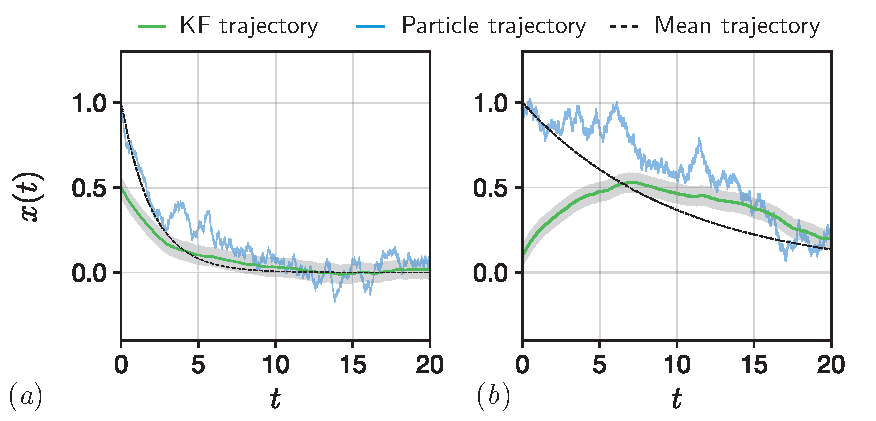
\includegraphics[width=\textwidth]{./figs/kbf.pdf}
    \caption{Evolution of the position of a Brownian particle in a harmonic potential (in blue) and its estimate using Kalman-Bucy filter (in green) when $\alpha(t) = \sigma(t) = 1$, in $(a)$ $f(t) = 0.5, \hat{x}(0) = 0.5, \beta(0) = 0.01$ and $(b)$ $f(t) = 0.1, \hat{x}(0) = 0.1, \beta(0) = 0.08$. The dashed line is the mean of state vector $\E[x(t)]=x_0 \exp(f t)$. Further details are available in the \href{https://github.com/sgangaprasath/KFTutorial/blob/main/KFTutorial.ipynb}{\texttt{python}}-notebook.}
    \label{fig:kbfFig}
\end{figure}

\section{Kalman filtering as recursive Bayesian estimation}
The problem of estimation is fundamentally an inverse problem
of obtaining the underlying system state from measurements,
whereas the known dynamics and measurement models specify the
forward relationship from the system state to the measurements.
In principle, the problem of obtaining the optimal state estimate
at any given time can be cast as a \emph{batch estimation} problem
solving for the state trajectory most likely to produce the observed
measurement sequence. This formulation is natural since the measurement sequence
constitutes the available data in the estimation problem.
However, the Kalman filter reformulates the batch estimation problem
into a recursive filtering problem, 
maintaining a running state estimate $\thh_k$ 
that is recursively updated with only a single incoming measurement $\m_k$ at 
time $k$, as opposed to working with
the entire (batch) measurement sequence $\m_1, \ldots, \m_k$.
This recursive structure of the Kalman filter opens up the
possibility for comparison with Bayesian estimation.
To this end, we first recall the Bayes rule given by
\begin{align*}
    p \left( \th \; | \; \m \right) = \frac{p \left( \th \right) p \left( \m  \; | \; \th \right)}{\int p \left( \th \right) p \left( \m  \; | \; \th \right) d\th }.
\end{align*}
Here $p \left( \th \; | \; \m \right)$ is the posterior probability
of the parameter $\th$ given the measurement $\m$, $p(\th)$ is the
prior probability on the parameter space and $p\left( \m  \; | \; \th \right)$ is the likelihood of the measurement $\m$ given the parameter $\th$.
Ignoring the normalization constant (which is automatically retrieved 
when the posterior is constrained to be a probability distribution), Bayes rule gives us the relation $p \left( \th \; | \; \m \right) \propto p \left( \th \right) p \left( \m  \; | \; \th \right)$.
Loosely interpreting Kalman filtering in Bayesian terms, the estimate propagation step of the Kalman filter propagates the state estimate (mean and covariance) from the previous time step to generate a 
prior for the current step, whereas the estimate update step
corrects the prior using the measurement residual to produce 
the posterior.

In Bayesian filtering, the current prior is obtained by propagation 
of the posterior from the previous time using the known system dynamics 
and is then corrected according to Bayes rule (using the current measurement and the likelihood function) to obtain the
current posterior, and the entire process is carried out recursively.
We will now show precisely that the recursive Bayesian estimator yields the Kalman filter when the underlying system dynamics is linear and the probability distributions of the noise (in the system dynamics and measurement model) are Gaussian.

\subsubsection*{Bayesian prior}
The prior probability for the current time $k$ is obtained by
forward propagating the posterior probability from the previous time $k-1$
using the system dynamics. Since the underlying probability distributions are
Gaussian (this can be verified from the fact that for any initial state of the system, the linear dynamics and Gaussian noise generate a sequence of 
states $\th_k$ which follow a Gaussian distribution for every $k$), 
this step involves forward propagating the mean and covariance of the posterior
from time $k-1$. The posterior mean at time $k-1$, denoted by $\thh_{k-1}$ 
is propagated by the dynamics to $\PhiB_{k-1} \thh_{k-1}$. Similarly, 
the prior covariance at time $k$ is obtained as $\p_k^{-} = \PhiB_{k-1} \p_{k-1} \PhiB_{k-1}^\top + \LambdaB_{k-1} \q_{k-1} \LambdaB_{k-1}^\top$,
to define the prior probability density as
\begin{align*}
    p_k \left( \th \; | \; \thh_{k-1} \right) \sim e^{ - \left( \th - \PhiB_{k-1} \thh_{k-1} \right)^\top {\p_k^{-}}^{-1}  \left( \th - \PhiB_{k-1} \thh_{k-1} \right)}.
\end{align*}
Note that the generation of the above prior merely involves
forward propagation through the system dynamics and is identical
to the estimates propagation step of the Kalman filter.

\subsubsection*{Likelihood}
The measurement model, with Gaussian noise of covariance $\S_k$ at time $k$, yields the likelihood function
\begin{align*}
    p_k \left( \m  \; | \; \th \right) \sim e^{ - \left( \m - \H_k \th \right)^\top \S_k^{-1}  \left( \m - \H_k \th \right)}.
\end{align*}

\subsubsection*{Posterior}
The posterior probability is then obtained by combining the prior probability 
and likelihood according to Bayes rule, and is given by
\begin{align*}
    p_k \left( \th  \; | \; \m_k, \thh_{k-1} \right) \sim e^{ - \left( \th - \PhiB_{k-1} \thh_{k-1} \right)^\top {\p_k^{-}}^{-1}  \left( \th - \PhiB_{k-1} \thh_{k-1} \right)} \cdot 
    e^{ - \left( \m_{k} - \H_k \th \right)^\top \S_k^{-1}  \left( \m_k - \H_k \th \right)}.
\end{align*}

We now compute the posterior mean using the fact that 
the mean of a Gaussian distribution is also its mode (and the only
critical point of its
probability density function). The posterior mean $\thh_{k}$
is then obtained as the solution to
\begin{align*}
    \frac{\partial}{\partial \th} \left. \left[ p_k \left( \th  \; | \; \m_k, \thh_{k-1} \right) \right] \right|_{\thh_{k}} = 0,
\end{align*}
which yields
\begin{align*}
    \frac{\partial}{\partial \th} \bigg[ ( \th - \PhiB_{k-1} \thh_{k-1} )^\top {\p_k^{-}}^{-1}  ( \th - \PhiB_{k-1} \thh_{k-1} ) \\
    + ( \m_k - \H_k \th )^\top \S_k^{-1}  ( \m_k - \H_k \th ) \bigg] \bigg|_{\thh_{k}} = 0.
\end{align*}
Solving the above, we get
\begin{align*}
    \thh_{k} = \left( {\p_k^{-}}^{-1} + \H_k^\top \S_k^{-1} \H_k \right)^{-1} \left( {\p_k^{-}}^{-1} \PhiB_{k-1} \thh_{k-1} + \H_k^\top \S_k^{-1} \m_k \right).
\end{align*}
It can be verified by the application of the Woodbury matrix identity 
that $\thh_{k}$ above can be expressed as
\begin{align*}
    \thh_{k} = \PhiB_{k-1} \thh_{k-1} + \K_k \left( \m_k - \H_k \PhiB_{k-1} \thh_{k-1} \right),
\end{align*}
where $\K_k = {\p_k^{-}} \H_k^\top \left( \S_k + \H_k {\p_k^{-}} \H_k^\top \right)^{-1}$. Note that the posterior mean $\thh_{k}$ and the gain $\K_k$ above are identical to the Kalman filter
updated estimate and the Kalman gain, respectively.
It can also be verified (we skip the calculation here) 
that the posterior covariance matches the
updated covariance from the Kalman filter.

\section{Beyond Kalman filter}
Following the advent of KF, several techniques were developed to accommodate the non-linearity of the dynamics and the non-gaussian aspects of the noise that often infect real world problems. Some of the popular techniques in literature include Extended Kalman Filter, Particle Filter, Unscented Kalman Filter, Ensemble Kalman Filter, Moving horizon estimation, and Recursive Bayesian estimation. Here we describe in brief the ideas behind Extended Kalman Filter and Particle Filter and point the interested reader to~\cite{simon2006optimal} for details of other techniques.

\subsubsection*{Extended Kalman Filter}
The process of state estimation under Kalman Filter is valid only for linear dynamics of the state vector.  Exact updates of the state vector for non-linear systems are in-general not available as the non-linearity results in a non-gaussian distribution of the state vector. An extension of the KF technique that is applied to non-linear systems with Gaussian noise is by locally linearizing the dynamics and is termed as the Extended Kalman Filter (shortened as EKF). This technique has been applied to several real-world scenarios and shown to perform well. However, EKF does not preserve the true mean and variance of the state vector and does not work for systems with multi-modal distributions.

\subsubsection*{Particle Filter}
Particle filtering is another technique used for state estimation when the underlying dynamics is non-linear and/or the process is non-gaussian. This technique uses particles to represent the posterior distribution of the state with the noisy measurements. Each particle has a likelihood weight that represents the probability of that particle/state being sampled from the probability density function of the state determined by sampling techniques such Monte Carlo methods. These weights and samples are then used to estimate the state of the system and as the number of samples becomes large, this distribution becomes equivalent to the true posterior distribution. Particle filtering technique is very popular as it makes little assumption about the underlying dynamics. However, this technique does not perform well when applied to high-dimensional dynamics and is often computationally expensive.

\section{Conclusion}
Kalman Filter was developed in 1960 first for aerospace applications and it played a pivotal role in the successful completion of the Apollo moon project, where it was used for trajectory estimation and navigation~\cite{grewal2010applications}. Post that, it was used for radar tracking of aircraft and was also critical in the development of the Global Positioning System (GPS) (which was then described as ``one enormous Kalman filter''~\cite{grewal2010applications}). Since its origin, KF has remained the go-to tool for sensor calibration and error correction. They have even been used in detecting constrictions of cerebral arterial blood vessels, detecting cancerous tumours, control of protein aggregation and in a gazillion other scenarios~\cite{grewal2010applications,fernandez2009extended,moreno2009kalman}.

In summary, we see that the Kalman filter is a powerful tool with wide ranging practical applications due to the recursive nature of the computations involved (no memory constraint), ease of implementation and a minimal set of assumptions required for its working. The foundation of the theory, however, is the famous least-squares fit which features in undergraduate textbooks. Several open questions remain till date as to the extension of the Kalman filter idea to non-linear/complex systems without simplifying assumptions that works for a wide range of dynamics. The physics community, in particular, is yet to dive into the estimation question and use some of the understandings of complex systems to answer the estimation question for systems that are physically constrained.


\bibliographystyle{unsrt}
\bibliography{references}

\end{document}